\documentclass{standalone}
\usepackage{tikz}

\usepackage{color}

\usetikzlibrary{arrows.meta}
\usetikzlibrary{calc}
\usetikzlibrary{shapes}
\usetikzlibrary{bending}
\usetikzlibrary{patterns}

\usepackage{gensymb}

\usepackage{pgfplots}
\usepgfplotslibrary{polar}

\begin{document}
		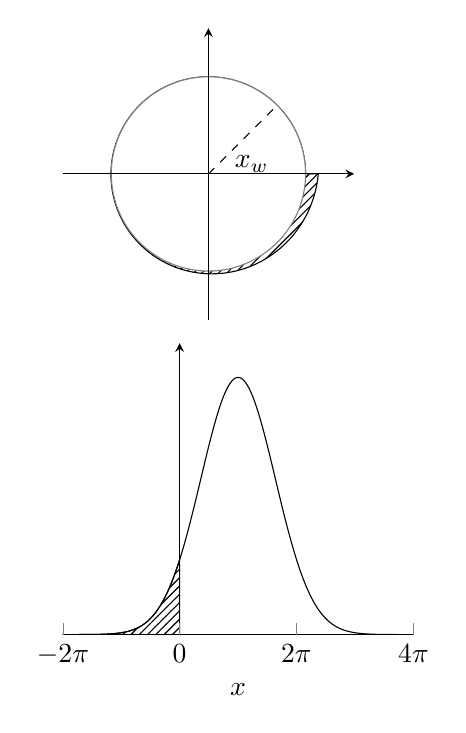
\begin{tikzpicture}[
	% scale=0.4,
	declare function={
		linf(\x) =      0.3*(1/2)*exp(-(1/8)*(\x-pi)*(\x-pi)); %N(mu=pi, sd=2) scale = 0.3
		func(\x) = 1 + (0.9*(1/2)*exp(-(1/8)*(\x-3*pi)*(\x-3*pi))); %wrappedN(mu=pi, sd=2) scale=0.5, k=0
	}
	]	
	
	\begin{axis}[
	scale=0.65,
	axis on top=true,
	unit vector ratio=1 1,
	axis x line=middle, axis y line=middle,
	xtick=\empty,
	ytick=\empty,
	xlabel=$x_w$,
	x label style={right=-13mm, above=-1mm},
	ymin=-1.5, ymax=1.5, 
	xmin=-1.5, xmax=1.5, 
	]
	
	\addplot[pattern=north east lines,data cs=polarrad, domain=0:2*pi,samples=300]{func(x)} \closedcycle;
	
	\addplot[samples=300, domain=0:2*pi,gray,fill=white]
	({cos(deg(x))}, {sin(deg(x))}) \closedcycle;
	
	
	%indication of angle
	\addplot[domain=0:0.5*1.41, dashed]{x};
	
	\end{axis}
	
	\begin{axis}[
	axis on top=true,
	yshift=-4cm,
	scale=0.65,
	axis x line*=middle, axis y line=middle,
	xtick=\empty,
	ytick=\empty,
	extra x ticks={-6.27,0,6.27,12.57},
	extra x tick labels={$-2\pi$,0,$2\pi$,$4\pi$},
	xlabel = $x$,
	xlabel near ticks,
	ymin=0, ymax=0.17,
	xmin=-2*pi, xmax=4*pi]
	
	%density on the full domain
	\addplot[domain=-2*pi:4*pi,samples=300]{linf(x)};
	
	%shaded area
	\addplot[pattern=north east lines, domain=-2*pi:0,samples=300]{linf(x)} \closedcycle;
	
	\end{axis}
	
	
	\end{tikzpicture}  
\end{document}